% !TEX TS-program = lualatex
% !TEX encoding = UTF-8

% This is a simple template for a LuaLaTeX document using gregorio scores.

\documentclass[letterpaper,12pt]{book} % use larger type; default would be 10pt

\input{header.inc}
\gresetheadercapture{commentary}{grecommentary}{string}

\geometry{letterpaper,outer=0.5in,inner=1.1in,top=0.5in,bottom=1in}

\begin{document}
\garamondbig

\printtitle{The Washing of the Feet (Mandatum or Maundy)}

\printtitle{I}
\greannotation{Ant.}
\greannotation{3.}
\gregorioscore{036_an--mandatum_novum--solesmes}

%\bigskip\bigskip
\printtitle{II}
\greannotation{Ant.}
\greannotation{4.}
\gregorioscore{037_an--postquam_surrexit--solesmes}

\vspace{1in}
\printtitle{III}
\greannotation{Ant.}
\greannotation{2.}
\gregorioscore{038_an--dominus_jesus--solesmes}

\vfill
\printtitle{IV}
\greannotation{Ant.}
\greannotation{5.}
\gregorioscore{039_an--domine_tu_mihi--solesmes}

\pagebreak
\printtitle{V}
\greannotation{Ant.}
\greannotation{4.}
\gregorioscore{040_an--si_ego_dominus--solesmes}

\printtitle{VI}
\vspace{-0.5\baselineskip}
\greannotation{Ant.}
\greannotation{7.}
\gregorioscore{040-1_an--in_hoc_cognoscent--solesmes}

\vfill
\printtitle{VII}
\vspace{-0.5\baselineskip}
\greannotation{Ant.}
\greannotation{7.}
\gregorioscore{041_an--maneant_in_vobis--solesmes}

\vfill

\pagebreak
\printtitle{VIII}
\greannotation{Ant.}
\greannotation{6.}
\gregorioscore{042_an--ubi_caritas--solesmes}

\begin{centering}
\vfill

\noindent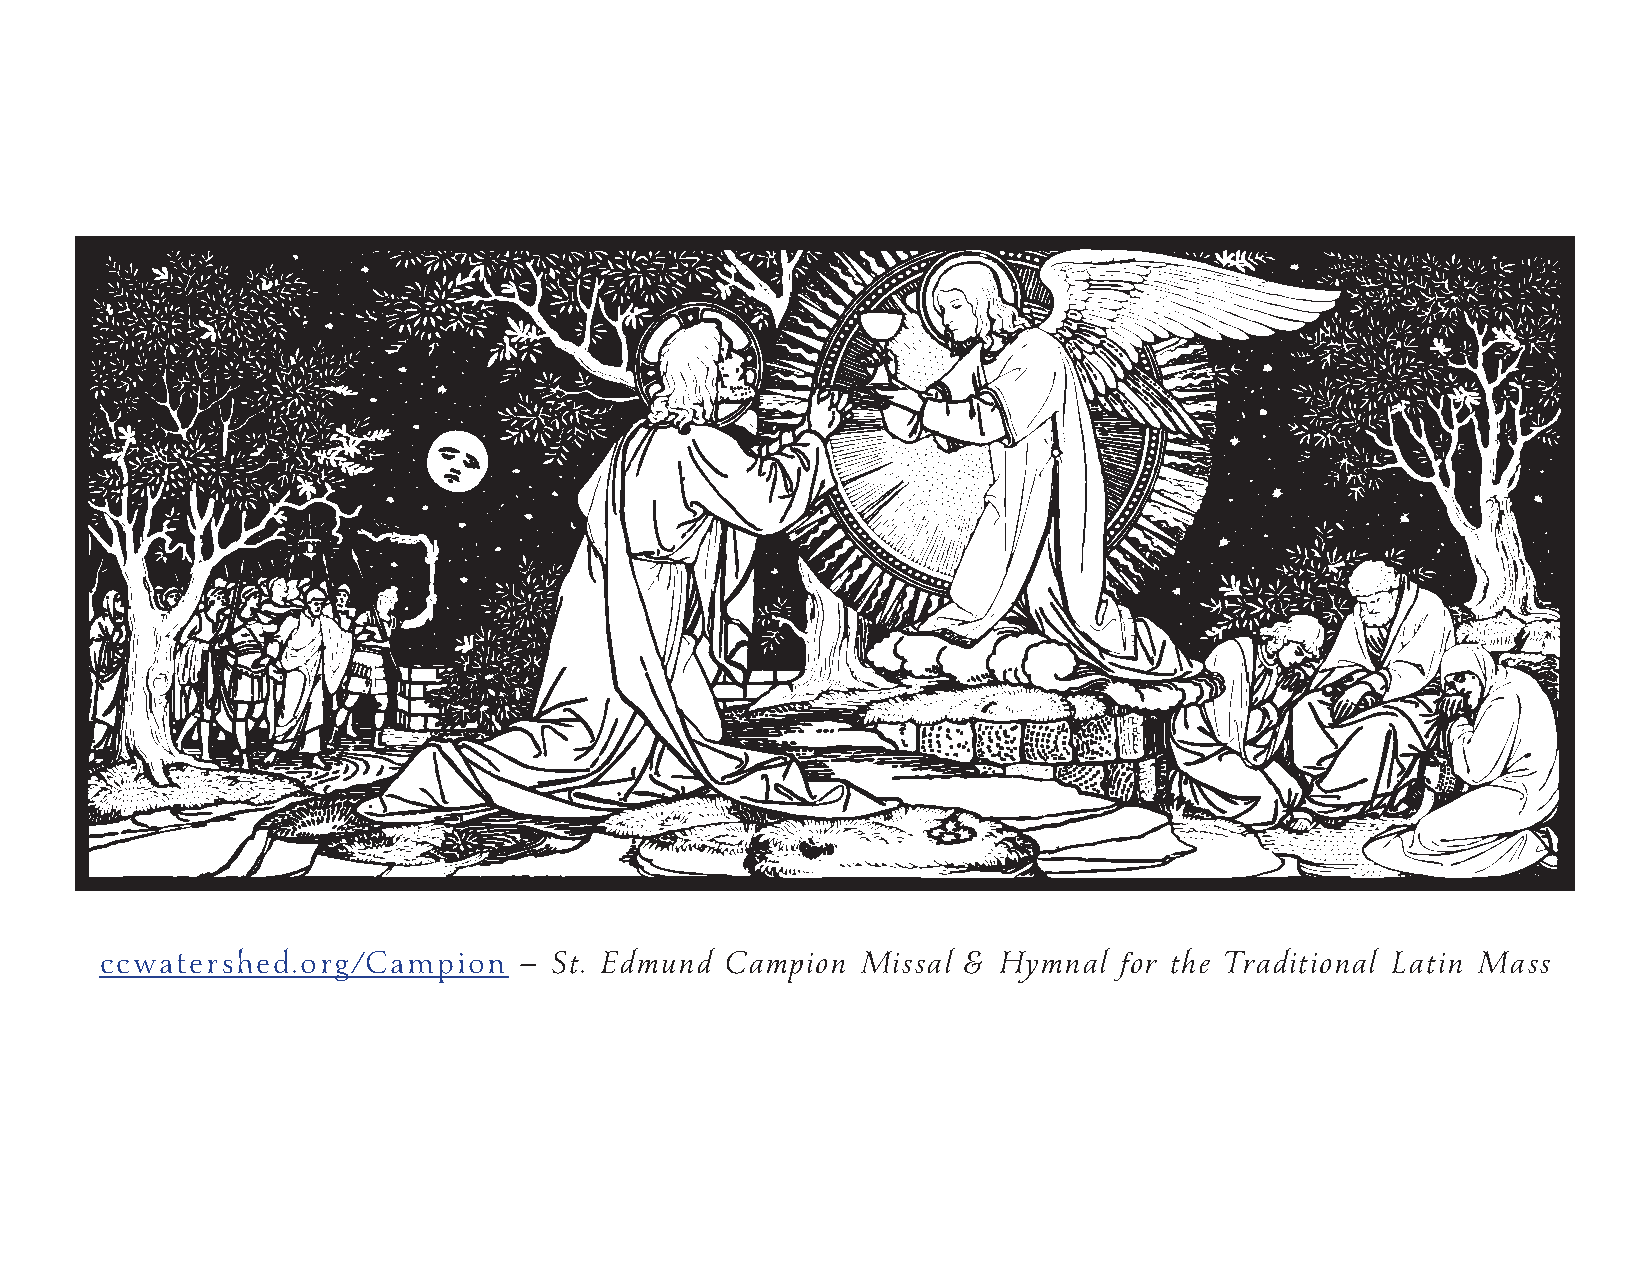
\includegraphics[clip,trim=0.5in 2.561in 0.5in 1.577in,width=\textwidth]{../040_10-03-11_0.pdf}

\vfill
\end{centering}


\end{document}